\chapter{シミュレーション結果}
\section{DCポテンシャル}
\Eq{rectangle_electrode}より,dc電圧を計算するためには電極モデルを矩形の形に分割する必要がある.Mathematica上における電極の分割の様子を\Fig{rect_electrode}に示す.
\begin{figure}[h]
	\begin{center}
		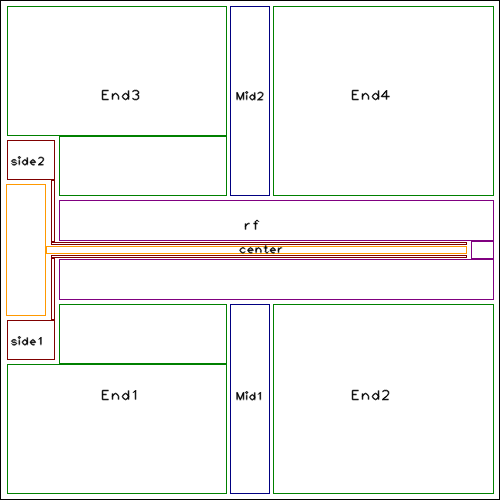
\includegraphics[width = 0.4\linewidth]{./simulation/figure/named_rect_electrode.png}
	\end{center}
	\caption{a}
	\label{fig:rect_electrode}
\end{figure}
各dc電極によってプレーナートラップ上の点$(x,y,z)$に形成される静電ポテンシャル$\Phi_{\rm DC}(x,y,z)$は,分割した各矩形が$(x,y,z)$に形成する静電ポテンシャルの重ね合わせで
\large
\begin{align}
	\Phi_{\rm DC}(x,y,z) = \phi_{\rm End1} + \phi_{\rm End2} + \phi_{\rm End3} &+ \phi_{\rm End4} + \phi_{\rm Mid1} + \phi_{\rm Mid2} \notag \\
	&+ \phi_{\rm Side1} + \phi_{\rm Side2} + \phi_{\rm center},
\end{align}
\normalsize
と表すことができる.
\begin{figure}[h]
	\begin{center}
		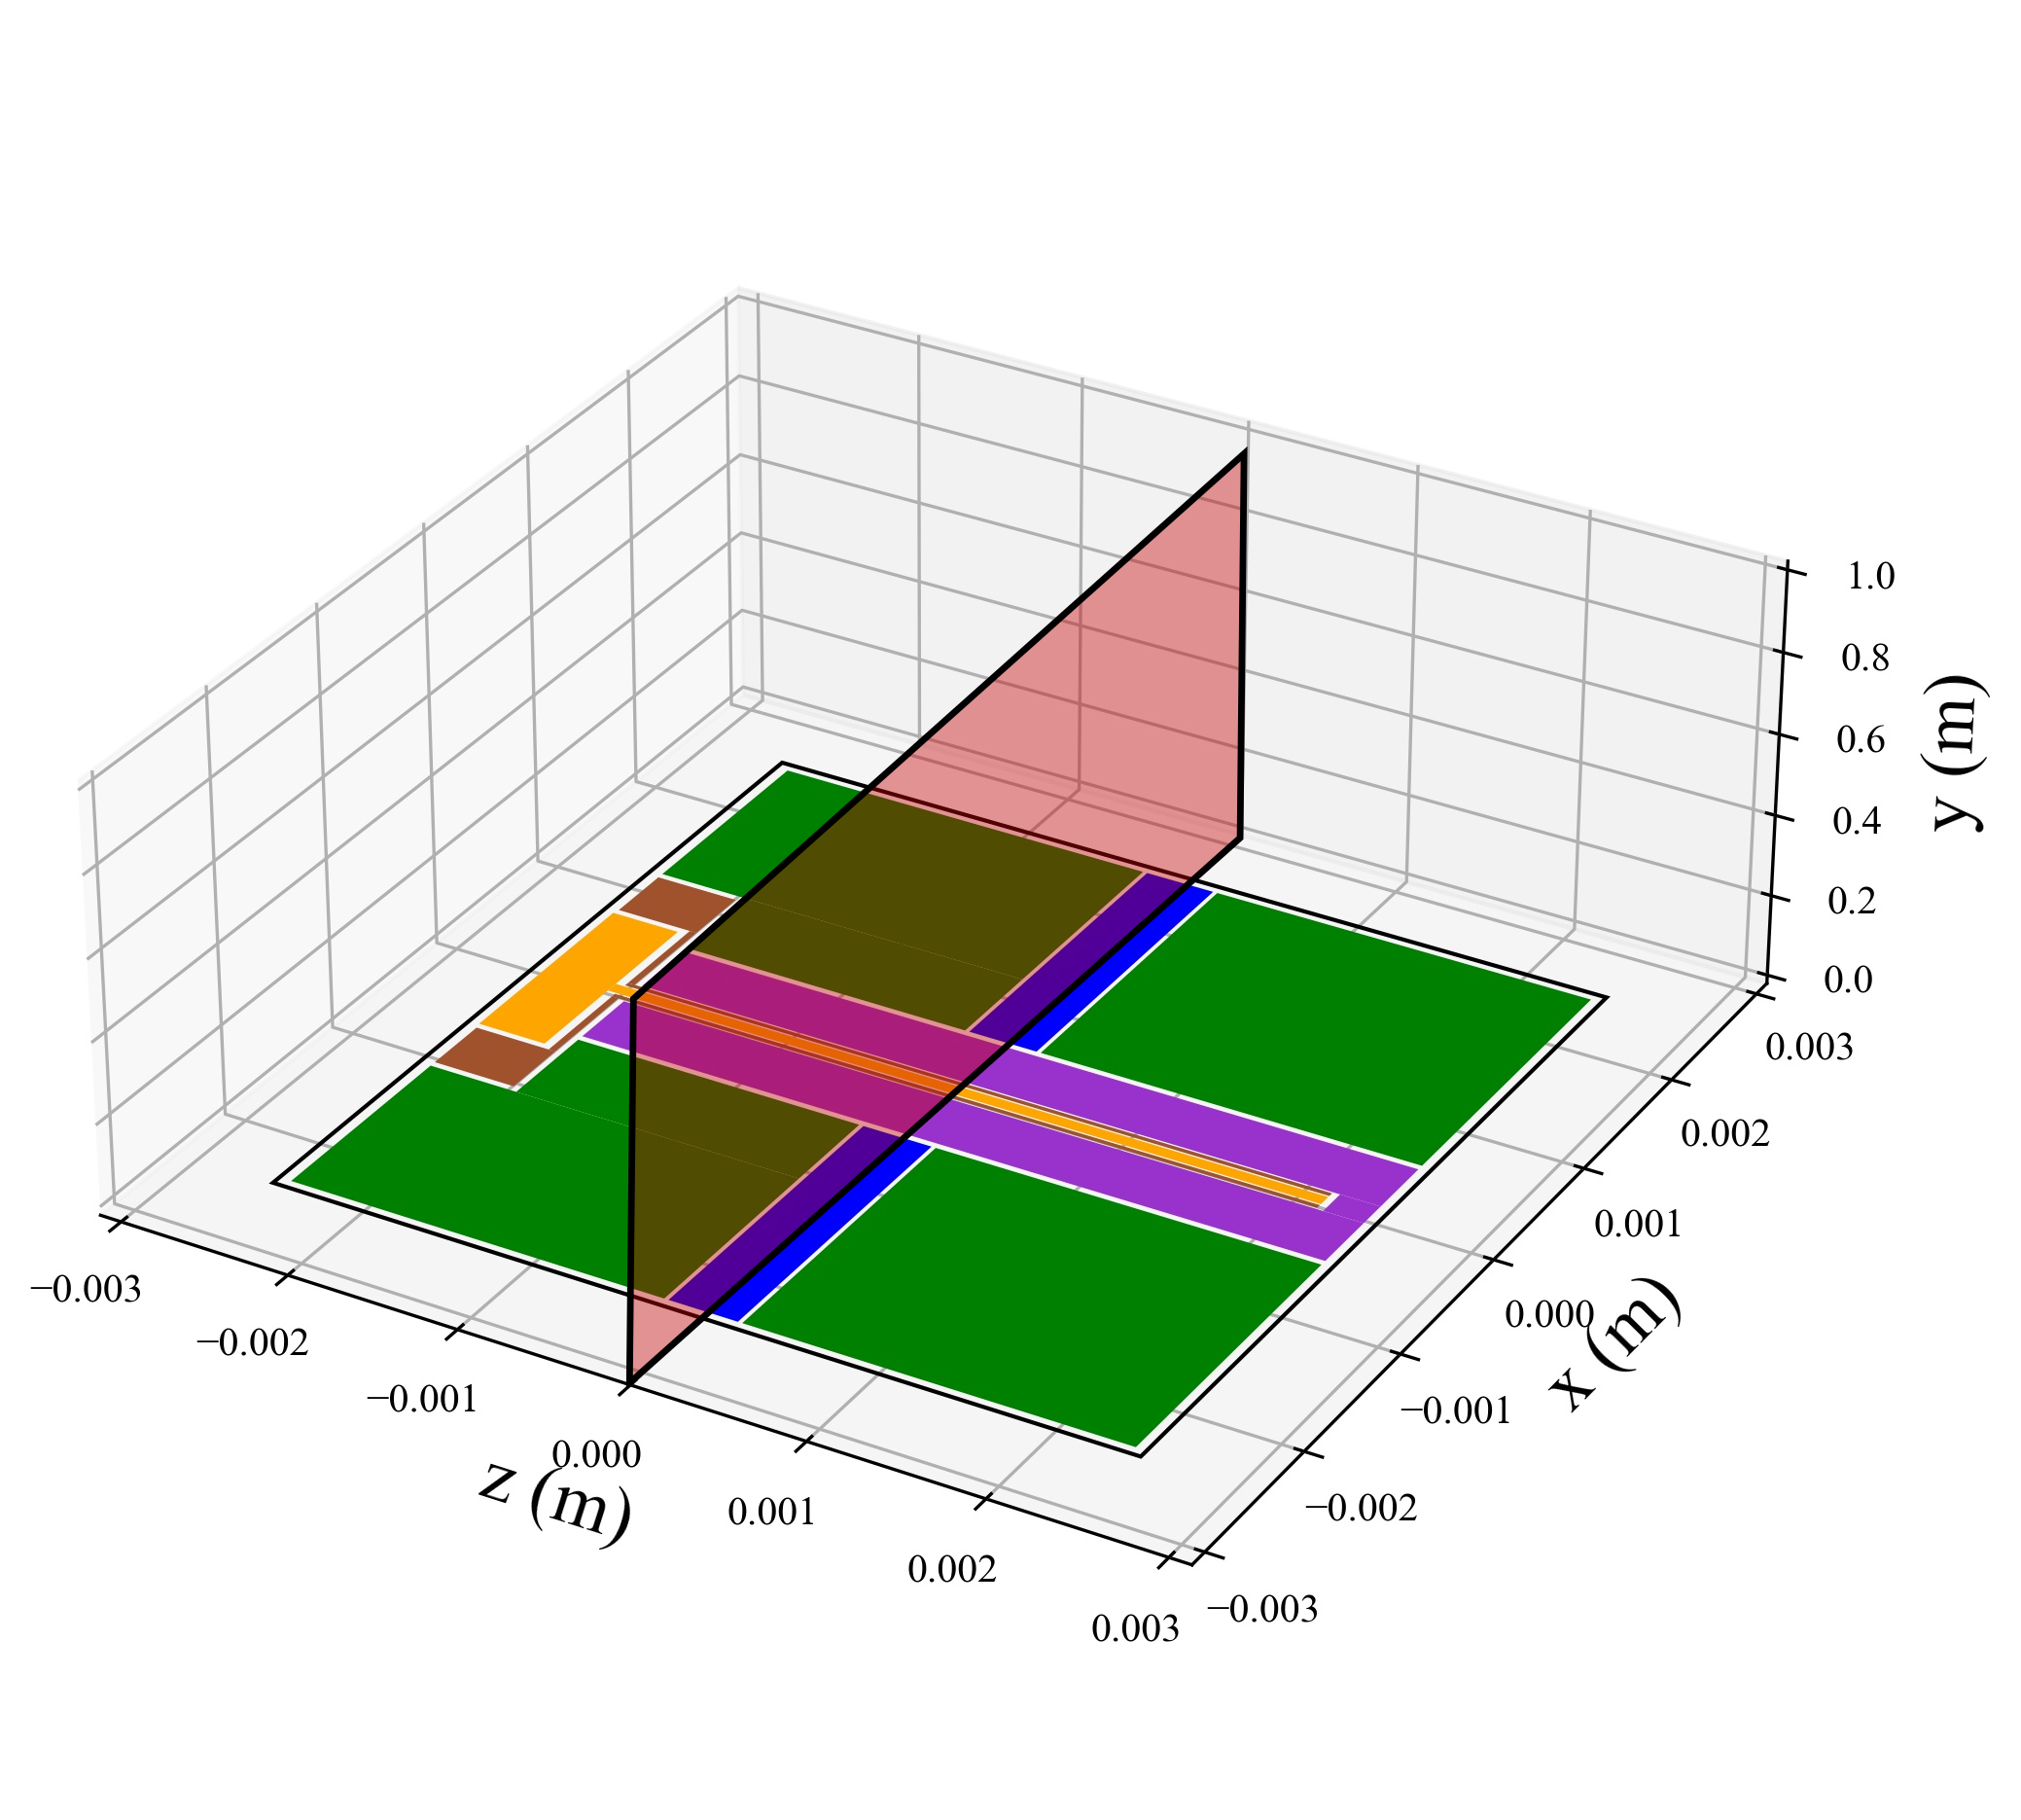
\includegraphics[width = 0.7\linewidth]{./simulation/figure/PlannarTrap_3D_z=0.png}
	\end{center}
\end{figure}
\begin{figure}[h]
	\begin{center}
		\begin{minipage}{0.45\linewidth}
			\begin{center}
				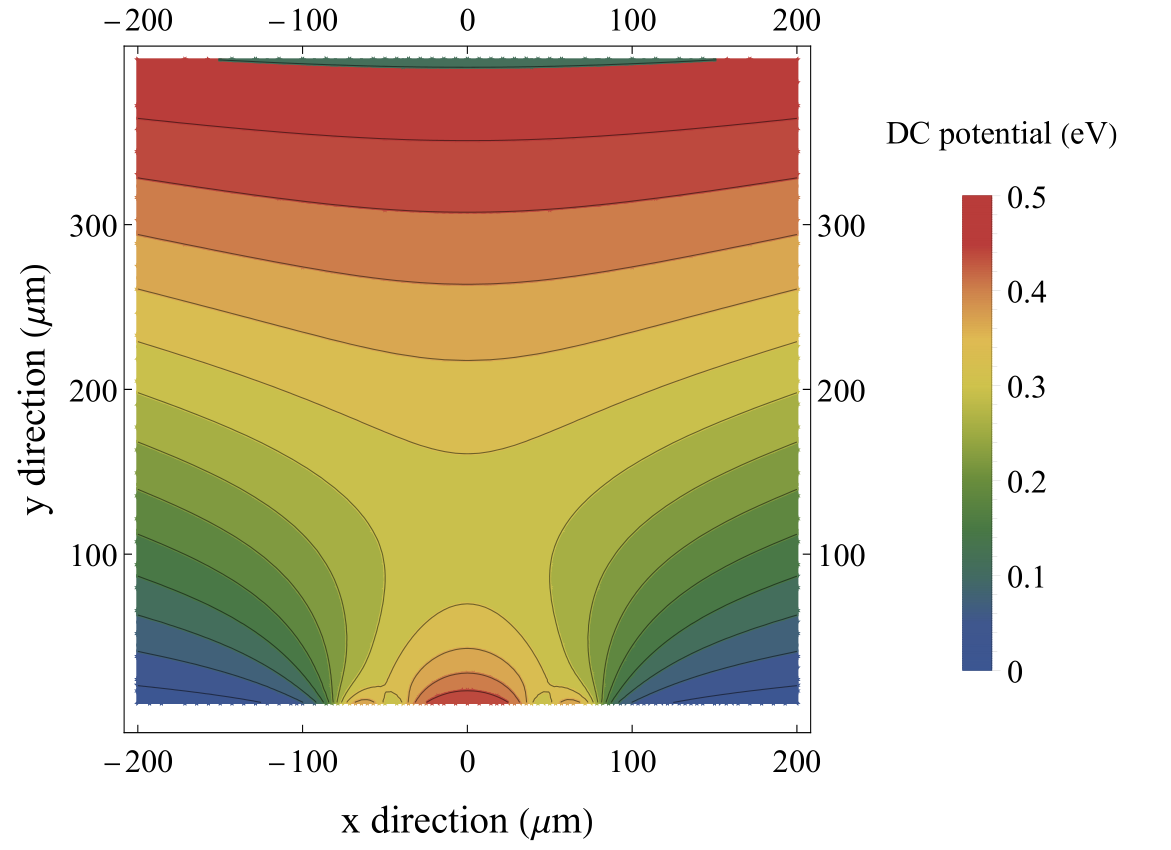
\includegraphics[width = 1.2\columnwidth]{./simulation/figure/dc_potential_example.png}
			\end{center}
		\end{minipage}
		\begin{minipage}{0.45\linewidth}
			\begin{center}
				\begin{tabular}{c|c} \hline \hline
					電極 & 印加電圧 ()V) \\ \hline
					End1 & 1.41 \\ \hline
					End2 & 1.41 \\ \hline
					End3 & 1.41 \\ \hline
					End4 & 1.41 \\ \hline
					Mid1 & -1.532 \\ \hline
					Mid2 & -1.532 \\ \hline
					Side1 & 0.222 \\ \hline
					Side2 & 0.222 \\ \hline
					center & 0.225 \\ \hline
				\end{tabular}
			\end{center}
		\end{minipage}
	\end{center}
\end{figure}
\section{Single-wellにおけるrf擬ポテンシャル}
\begin{figure}[h]
	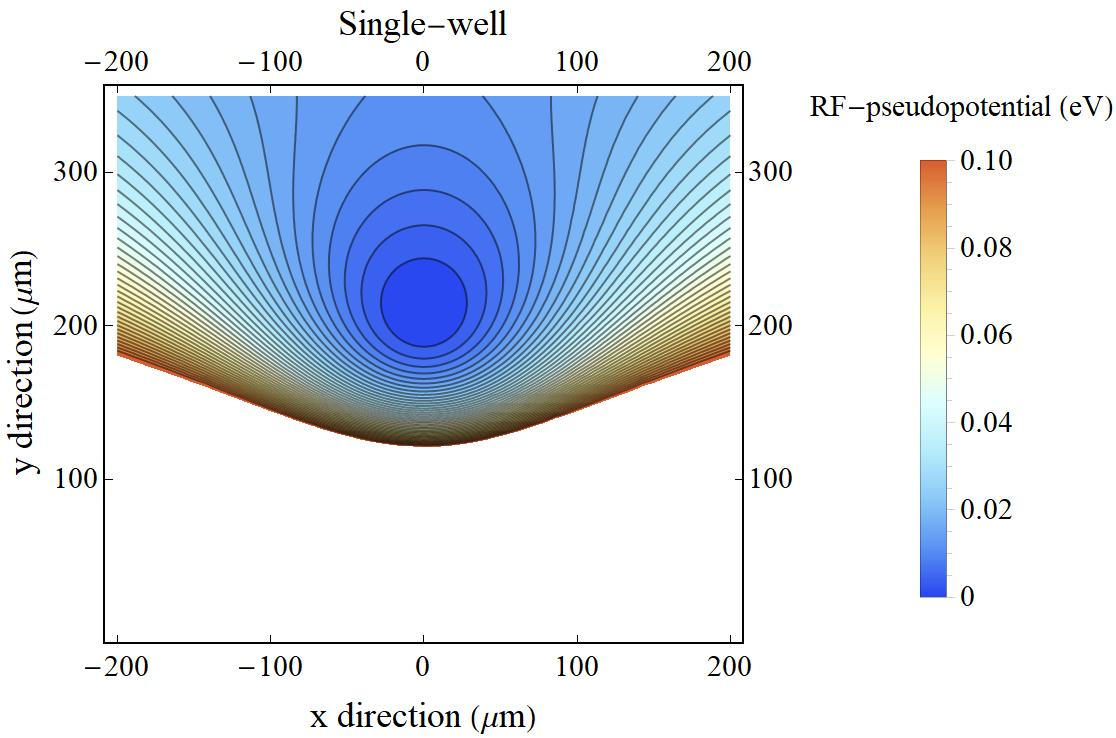
\includegraphics[width = 0.7\linewidth]{./simulation/figure/Single-well_Contour_xy@z=0.jpg}
	\caption{single-well}
	\label{fig:single-well_example}
\end{figure}
\section{Double-wellにおけるrf擬ポテンシャル}
\begin{figure}[h]
	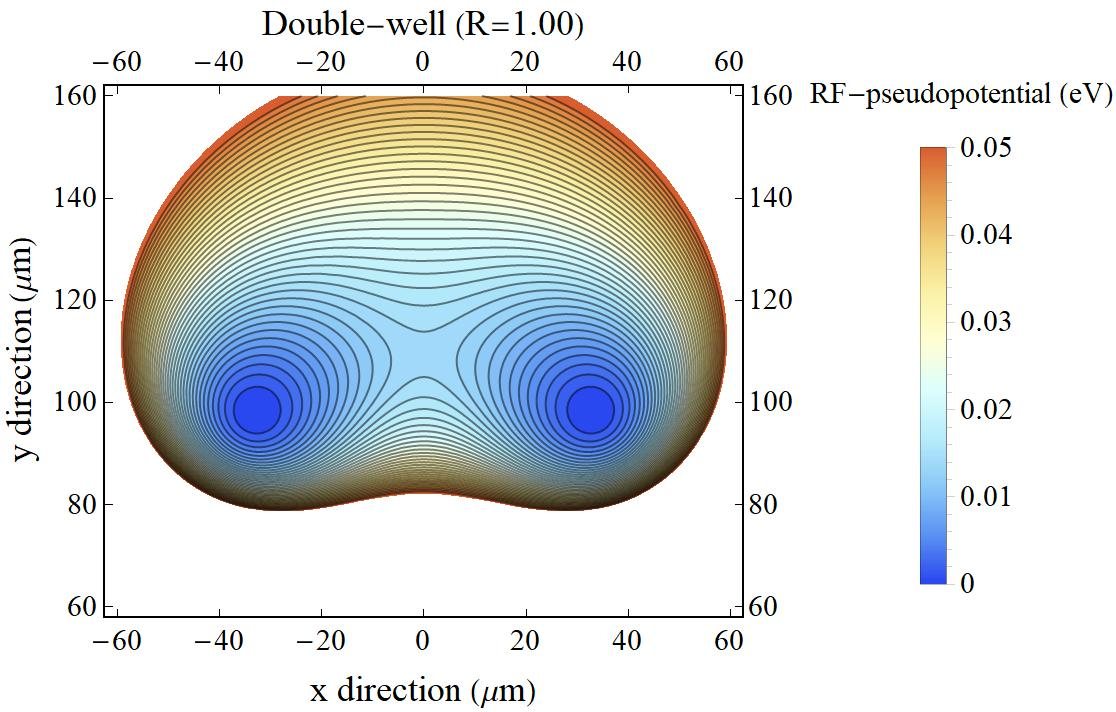
\includegraphics[width = 0.7\linewidth]{./simulation/figure/Double-well_Contour_xy_R=100.jpg}
	\caption{double-well}
	\label{fig:double-well_example}
\end{figure}